\section{Case study: outperforming by being diverse only when necessary}\label{sec:how_work}
We design $\mathtt{Pac}$-$\mathtt{Men}$ shown in Fig.~\ref{fig:pec_man} to demonstrate how our approach works. In this task, four agents are initialized at the center room and can only observe a 5 × 5 grid around them. Three dots are initialized randomly in each edge room. To make this environment more challenging, paths to different rooms have different lengths, which are down : left : up : right = 4 : 8 : 12 : 8. Three out of four paths are outside agents' observation scope, which brings about the difficulty of exploration. Dots will refresh randomly after all rooms are empty. An ineffective competition between agents occurs when they come together in one room. The total environmental reward is the number of dots eaten in one step or -0.1 if no one eats dots. The time limit of this environment is set to 100 steps.

\begin{figure*}[ht]
\centering
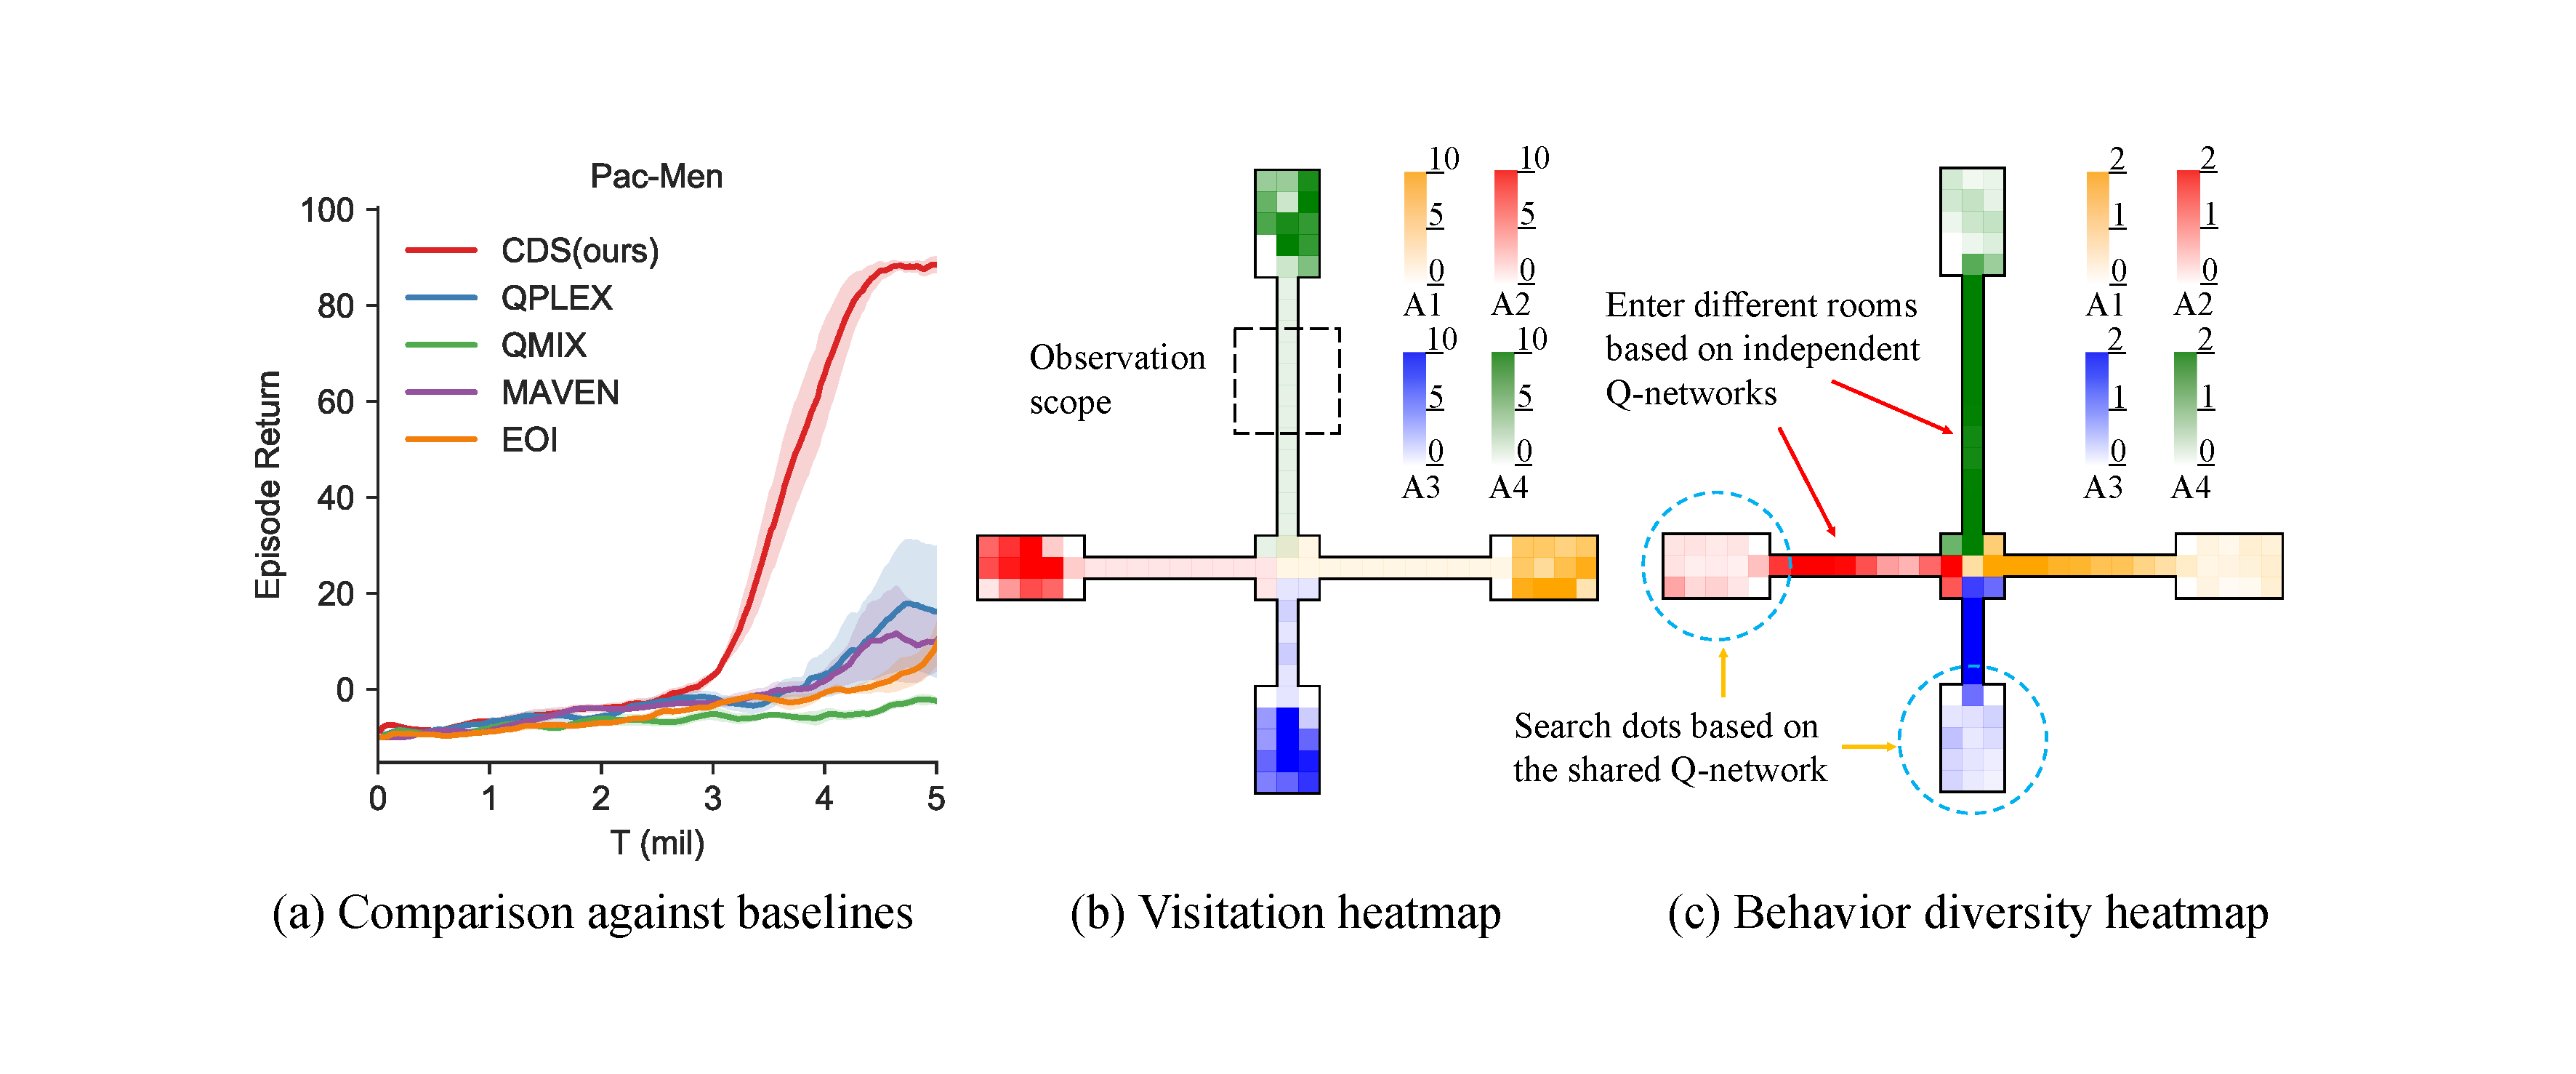
\includegraphics[width=1.\linewidth]{pic/Pac-Men.pdf}
\caption{Why does our method work? The balance between identity-aware diversity and experience sharing encourages sophisticated strategies.}
\label{fig:pec_man}
\end{figure*}
%\includegraphics[height=0.31\linewidth]{pic/pacmen_plot}
%\includegraphics[height=0.31\linewidth]{pic/pacmen-large}

%\begin{wrapfigure}[16]{r}{0.5\linewidth}
%    \vspace{0.05cm}
%	\centering%
%	\includegraphics[width=\linewidth]{pic/pacmen_pos_ratio.pdf}
%	\caption{Heat maps of visit frequency and the ratio of standard deviation (SD) for four agents.}
%	\label{fig:pacmen_pos_ratio}
%\end{wrapfigure}

Fig.~\ref{fig:pec_man}-middle demonstrates the learned strategies of our approach, with a heatmap showing the visitation number. Driven by the objective of mutual information between individual trajectory and identity, agents achieve diversity and scatter in different rooms to eat dots. We further analyze the role of independent and shared Q-functions during different stages in Fig.~\ref{fig:pec_man} right. We visualize the value of $SD(Q_i^I(\cdot))/SD(Q^S(\cdot))$, where SD denotes the standard deviation (SD) of Q values for different actions. A higher SD ratio indicates the independent Q-functions play a leading role, while a lower SD ratio indicates the shared Q function's domination.

We notice that the SD ratio is considerably larger in the central room and four paths than in four edge rooms. This observation means that agents use independent Q networks to reach different rooms while use the shared Q network to search for dots in them. The result shows that our method achieves a good balance between diversity and knowledge sharing. Taking this advantage, our approach outperforms baselines (Fig.~\ref{fig:pec_man} left, baselines are introduced in Sec.~\ref{experiment}). Other methods, such as variational exploration (MAVEN~\cite{mahajan2019maven}) and individuality emergence (EOI~\cite{jiang2020emergence}), are slower to learn optimal strategies.

%all baselines cannot effectively forbid agents to eat dots in a single room simultaneously and thus significantly underperform our method (Fig.~\ref{fig:pec_man} left).

% Meanwhile, almost all knowledge that can be shared, searching for dots to eat, are shared among agents. These impressive characteristics of our approach are urgently needed to emerge sophisticated cooperation strategies and broaden MARL to more challenging scenarios.
% The experiment result shows that our approach can precisely guide agents to adaptively and reasonably choose whether to use shared knowledge or excute their own diverse policies.